% LEFT COLUMN: the agent and the data.
\card{2.5}{21.6}{36.7}{23.0}{1}{Start simple: one model, two tools}
\txt{3.7}{25.1}{34.3}{ink}{24}{\textbf{QwQ-32B} does everything itself: it reasons, picks the next action, and summarizes the pages it reads.
  No external model is called.}
% Agent loop, redrawn for the poster.
\boxtext{3.7}{28.3}{7.4}{6.6}{pale}{21}{\textbf{Question}\\+\\\textbf{history}\\[1mm]{\fs{18}{21}\textcolor{muted}{analyses, actions, tool results}}}
\draw[arrow] (11.3,31.6)--(12.8,31.6);
\filldraw[fill=mint,draw=line,line width=1pt,rounded corners=3mm] (13.0,28.0) rectangle (24.6,37.0);
\node[text=navy,font=\fs{25}{30}\bfseries] at (18.8,29.0) {QwQ-32B};
\boxtext{13.6}{30.0}{10.4}{2.0}{lavender}{21}{\textbf{Reason}\enspace\textcolor{muted}{(not kept)}}
\boxtext{13.6}{32.3}{10.4}{2.0}{white}{21}{\textbf{Analyze}\enspace\textcolor{muted}{(kept)}}
\boxtext{13.6}{34.6}{10.4}{2.0}{peach}{21}{\textbf{Act}}
\boxtext{26.8}{28.0}{11.2}{2.7}{pale}{21}{\textbf{search}\enspace$\to$ snippets + URLs}
\boxtext{26.8}{31.2}{11.2}{2.7}{pale}{21}{\textbf{access}\enspace$\to$ page $\to$ summary}
\boxtext{26.8}{34.4}{11.2}{2.6}{lavender}{21}{\textbf{answer}\enspace$\to$ done}
\draw[arrow] (24.6,35.6)--(26.6,29.35);
\draw[arrow] (24.6,35.6)--(26.6,32.55);
\draw[arrow] (24.6,35.6)--(26.6,35.7);
\draw[arrow,rounded corners=4mm] (38.0,29.35)--(38.6,29.35)--(38.6,38.3)--(7.4,38.3)--(7.4,35.1);
\draw[line width=3pt,draw=blue] (38.0,32.55)--(38.6,32.55);
\node[fill=white,inner sep=2mm,text=muted,font=\fs{20}{24}] at (22.5,38.3) {results join the history \;$\cdot$\; up to 128 turns};
\boxtext{3.7}{39.6}{16.7}{1.9}{mint}{21}{\textcolor{teal}{$\checkmark$}\ \textbf{one model} does everything}
\boxtext{21.3}{39.6}{16.7}{1.9}{mint}{21}{\textcolor{teal}{$\checkmark$}\ \textbf{no external} model API}
\txt{3.7}{42.0}{34.3}{muted}{21}{Lengthy reasoning is dropped from the history; webpages are summarized in 10k-character chunks.}
\card{2.5}{45.7}{36.7}{36.9}{2}{Give it questions worth searching}
\txt{3.7}{49.2}{34.3}{ink}{24}{Easy questions teach shortcuts, so the data is made hard on purpose: a synthesis agent rewrites seed questions until they truly need search.}
% Synthesis loop, redrawn.
\boxtext{3.7}{52.2}{7.4}{4.0}{pale}{21}{\textbf{Seed QA}\\+ facts}
\draw[arrow] (11.3,54.2)--(12.4,54.2);
\boxtext{12.6}{52.2}{7.4}{4.0}{mint}{21}{\textbf{Inject}\\a sourced fact}
\draw[arrow] (20.2,54.2)--(21.3,54.2);
\boxtext{21.5}{52.2}{7.4}{4.0}{lavender}{21}{\textbf{Fuzz}\\a telling detail}
\draw[arrow] (29.1,54.2)--(30.2,54.2);
\boxtext{30.4}{52.2}{7.6}{4.0}{peach}{21}{\textbf{Verify}\\3 checks}
\draw[arrow,rounded corners=4mm] (34.2,56.3)--(34.2,57.3)--(7.4,57.3)--(7.4,56.4);
\node[fill=white,inner sep=2mm,text=muted,font=\fs{20}{24}] at (20.8,57.3) {keep the new question only if it passes, then repeat};
% Worked example from the paper's figure.
\filldraw[fill=pale,draw=line,line width=1pt,rounded corners=3mm] (3.7,58.5) rectangle (38.0,69.2);
\foreach \yy/\tag/\col/\q in {
  59.1/SEED/pale/{How many years was Daniel Charbonell's contract with the San Francisco Giants when he signed in 2014?},
  61.6/INJECT/mint/{How many years was the contract signed in 2014 by \textbf{the Cuban outfielder who played for the San Jose Giants}?},
  64.1/FUZZ/lavender/{How many years was Daniel Charbonell's contract with the San Francisco Giants when he signed in \textbf{the early 2010s}?}}{%
  \filldraw[fill=\col,draw=line,rounded corners=2mm] (4.3,\yy) rectangle ++(4.6,1.3);
  \node[text=navy,font=\fs{18}{21}\bfseries] at (6.6,\yy+0.65) {\tag};
  \txt{9.4}{\yy}{28.1}{ink}{20}{\q}}
\txt{4.3}{66.7}{33.4}{ink}{20}{\textbf{Answer:} four years.\enspace \textbf{Uniqueness check:} could ``two years'' also be correct? If so, the question is rejected.}
\chip{3.7}{70.0}{10.9}{4.0}{pale}{304k$\to$16k}{hard open-source QA kept}
\chip{15.4}{70.0}{10.9}{4.0}{lavender}{25.6k}{synthesized QA pairs}
\chip{27.1}{70.0}{10.9}{4.0}{mint}{3 checks}{quality, difficulty, uniqueness}
\txt{3.7}{74.8}{34.3}{ink}{24}{\bfseries Then a two-stage curriculum}
\boxtext{3.7}{76.6}{15.0}{4.6}{pale}{22}{\textbf{Stage 1}\\mixed difficulties\\[1mm]learn basic tool use}
\draw[arrow] (19.1,78.9)--(22.6,78.9);
\boxtext{23.0}{76.6}{15.0}{4.6}{mint}{22}{\textbf{Stage 2}\\tasks needing $\ge5$ tool calls\\[1mm]learn deeper search}
% ===================================================================
% MIDDLE COLUMN: the training system and the learning signal.
\card{41.1}{21.6}{36.7}{34.8}{3}{Let long rollouts run free}
\txt{42.3}{25.1}{34.3}{ink}{24}{Hard questions need long searches, and long searches stall batch training.
  ASearcher runs rollouts of up to \textbf{128 actions} concurrently and trains as soon as enough of them finish.}
% Timeline, redrawn: batch generation vs. fully asynchronous RL.
\txt{42.3}{27.9}{34.3}{ink}{23}{\textcolor{red!70!black}{\bfseries$\times$}\ \textbf{Batch generation:} everyone waits for the slowest trajectory}
\foreach \a/\b in {43.0/48.6,48.9/54.0}{\fill[violet!45,rounded corners=1mm] (\a,29.4) rectangle (\b,30.5);}
\fill[pattern=north east lines,pattern color=muted!60] (54.3,29.4) rectangle (69.8,30.5);
\node[fill=white,inner sep=1mm,text=muted,font=\fs{20}{24}\bfseries] at (62.05,29.95) {GPUs idle};
\fill[violet,rounded corners=1mm] (43.0,30.9) rectangle (69.8,32.0);
\node[text=white,font=\fs{20}{24}\bfseries] at (56.4,31.45) {one long trajectory};
\boxtext{70.2}{29.4}{6.4}{2.6}{peach}{21}{\textbf{train}}
\txt{42.3}{33.3}{34.3}{ink}{23}{\textcolor{teal}{\bfseries$\checkmark$}\ \textbf{Fully asynchronous:} generation never stops; training never waits}
\foreach \a/\b in {43.0/48.3,48.6/53.9,54.2/59.5,59.8/65.1,65.4/70.7,71.0/76.4}{\fill[violet!45,rounded corners=1mm] (\a,34.8) rectangle (\b,35.9);}
\fill[violet,rounded corners=1mm] (43.0,36.3) rectangle (69.8,37.4);
\node[text=white,font=\fs{20}{24}\bfseries] at (56.4,36.85) {the same long trajectory};
\fill[violet!45,rounded corners=1mm] (70.1,36.3) rectangle (76.4,37.4);
\foreach \a/\l in {48.0/N,59.2/N+1,70.2/N+2}{\boxtext{\a}{38.0}{6.2}{1.9}{peach}{20}{\textbf{train} \l}}
\draw[-{Stealth[length=4mm]},line width=2pt,draw=muted] (43.0,40.5)--(76.4,40.5);
\node[anchor=east,text=muted,font=\fs{20}{24}] at (76.4,41.2) {time};
\txt{42.3}{40.9}{26}{muted}{21}{A long trajectory simply spans several policy versions.}
\node[anchor=north west,inner sep=0] at (42.3,43.4) {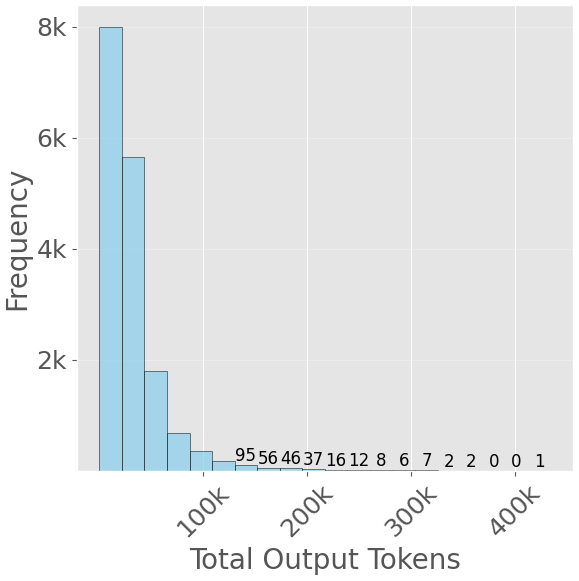
\includegraphics[width=11.4cm]{figures/fig4_lengths_crop.png}};
\filldraw[fill=pale,draw=line,line width=1pt,rounded corners=3mm] (54.7,43.4) rectangle (76.6,55.3);
\txt{55.5}{44.1}{20.4}{teal}{24}{\bfseries Why the tail matters}
\txt{55.5}{46.2}{20.4}{ink}{21}{%
  \textcolor{teal}{$\blacktriangleright$}\ Trajectory lengths are \textbf{long-tailed}: most stay below 100k tokens, a few approach 400k (left, training steps 290--310).\\[2.5mm]
  \textcolor{teal}{$\blacktriangleright$}\ A synchronous batch would wait for that tail.\\[2.5mm]
  \textcolor{teal}{$\blacktriangleright$}\ Asynchronous training lets finished trajectories go straight to the next update.}
